\documentclass[a4paper,10pt,twocolumn]{article}

\usepackage[utf8]{inputenc}
\usepackage[T1]{fontenc}
\usepackage{lmodern}  % makes ligatures copy-pasteable

\usepackage[ngerman]{babel}

\usepackage{hyperref}

\usepackage{amsmath}
\usepackage{xcolor}

\usepackage{epsfig}
\usepackage{epstopdf}

\usepackage{gensymb}

\title{Simulation Rohrbruch Gasverteilnetz}
\author{}
\date{}

\begin{document}

\maketitle

\section{Problemstellung}

\subsection{Rohrsegment mit Leck}

Diese Betrachtung bezieht sich auf ein Rohrsegment mit Leckagestelle, siehe Abb.~\ref{fig:bruch}.

\begin{figure}[hbp]
\centering
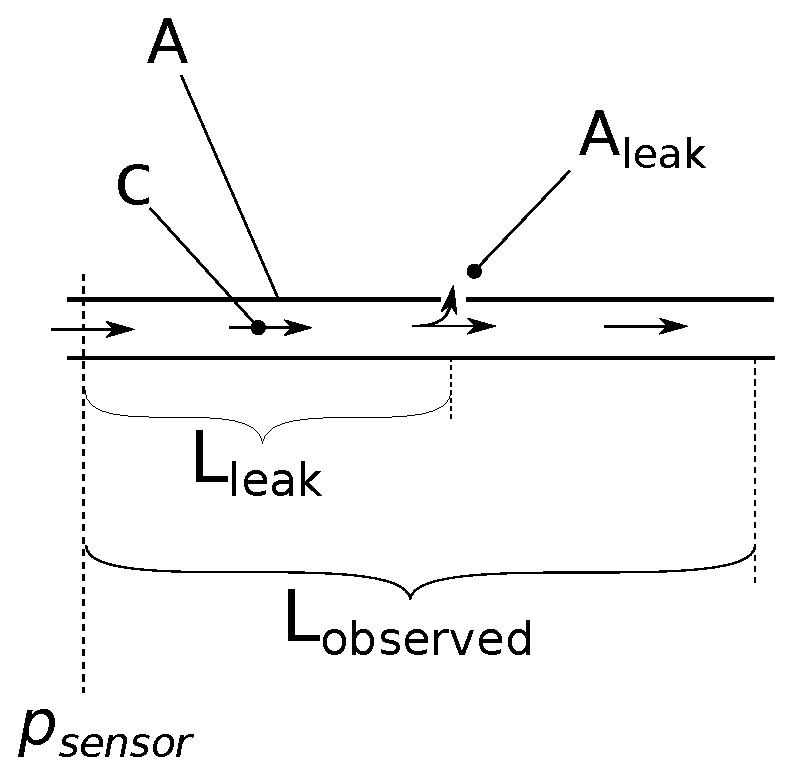
\includegraphics[width=0.9\hsize]{bruch.eps}
\caption{Rohrsegment mit Leckagestelle}
\label{fig:bruch}
\end{figure}

Es handelt sich um einen Rohrabschnitt mit konstanter Querschnittsfläche $A$, durch welchen einem Gas mit nominaler Geschwindigkeit $c$ strömt. Betrachtet wird ein Abschnitt der Länge $L_\mathit{observed}$, bei Lauflänge $L_\mathit{leak}$ ist ein Leck mit einer Querschnittsfläche $A_\mathit{leak}$.

Am Anfang des Segments befindet sich ein Sensor, welcher Eigenschaften der Rohrströmung misst, im gegebenen Fall den statischen Druck $p_\textit{sensor}$.

\subsection{Problem-Parameter}

Das Strömungsmedium ist Methan. Die Fliessgeschwindigkeit ist $\approx 10\,\mathrm{m/s}$. Der Rohrinnendruck ist $\approx 60\pm 10\,\mathrm{bar}$. Die Rohrinnentemperatur ist $\approx 10\,\mathrm{\degree C}$. Die Länge $L_\mathit{observed}$ ist $\approx 500 \ldots 1000 \,\mathrm{m}$.

\subsection{Problem-Frage}

Wie ändert sich die Messung an der Sensor-Stelle, wenn eine Leckagestelle $A_\mathit{leak}$ bzw. $L_\mathit{leak}$ plötzlich auftritt? Lassen sich solche z.B. durch Bauarbeiten verursachten Schäden detektieren durch solche Sensoren detektieren, und wie reagieren die Sensoren im jeweiligen Fall?

\section{Modellierung}

\subsection{Modellierung des Umsystems}

Die Modellierung zielt unter anderem darauf ab, das Umsystem, in diesem Fall die Welt vor und nach dem betrachteten Rohrsegment, realitätsnah nachzubilden.

\begin{figure}[hbp]
\centering
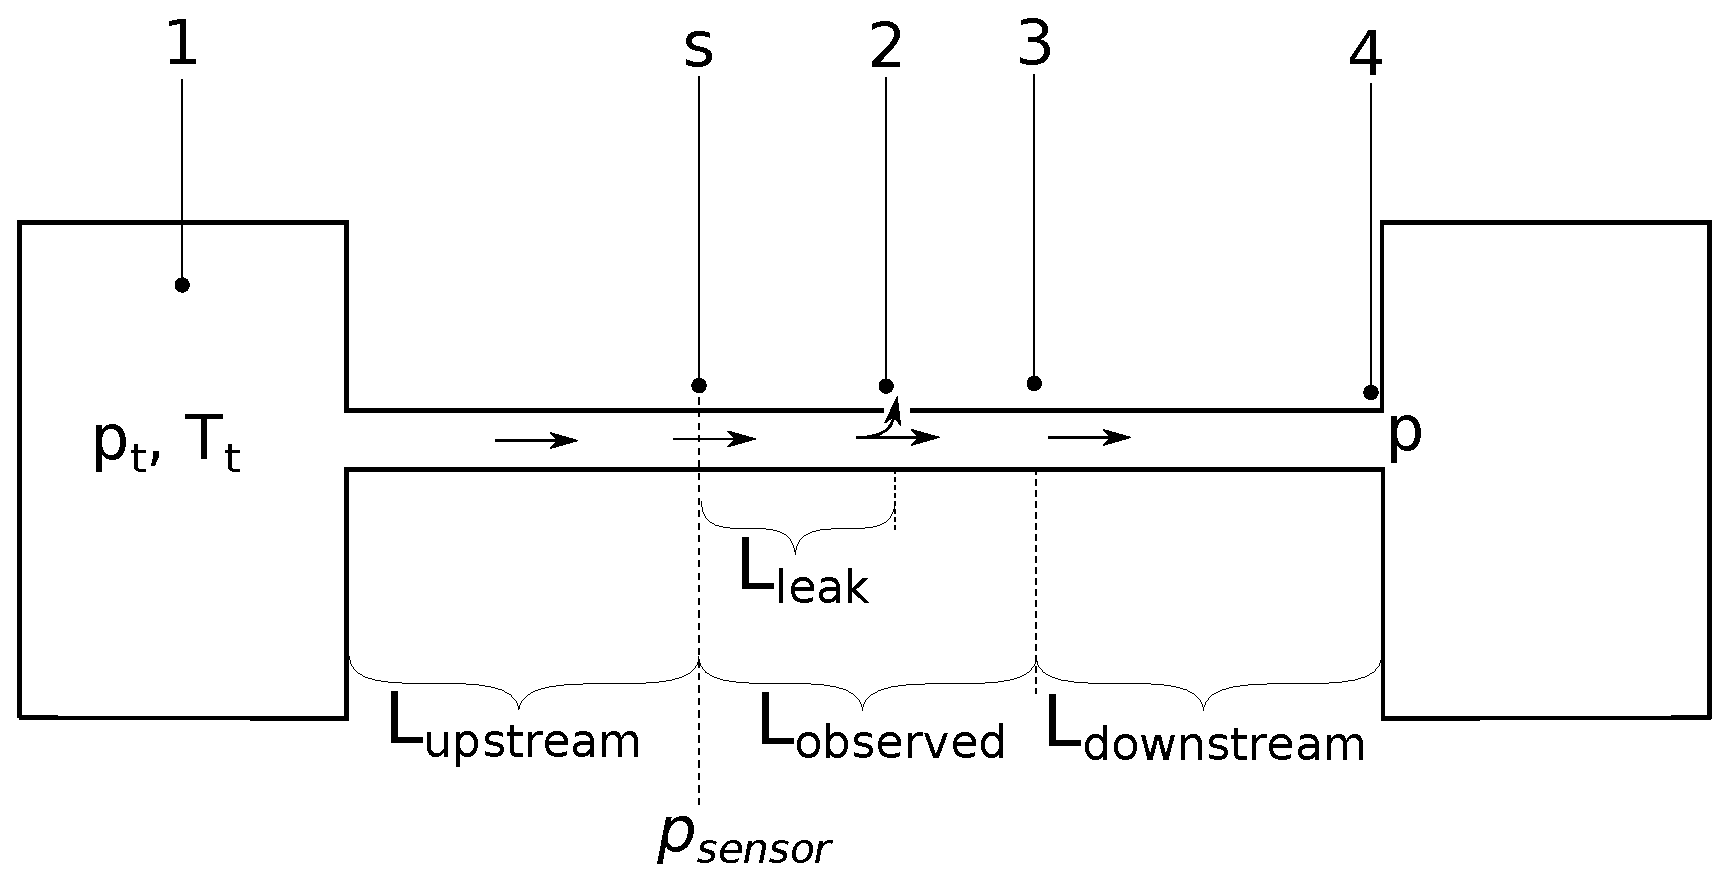
\includegraphics[width=0.9\hsize]{model.eps}
\caption{Modellierung}
\label{fig:model}
\end{figure}

Es wird zwecks Modellierung angenommen, dass sich stromauf und stromab jeweils ein Gascontainer befindet. Es wird angenommen, dass diese Container ein unendliches Volumen haben und ausgeglichen sind\footnote{Damit ist gewährleistet, das weiterer Aus- und Zufluss von Gas den Zustand des Containers nicht verändern, und damit die Randbedingungen beliebig lange stabil sind. Kurzzeitig ist dieses Modell in jedem Fall gültig; falls dieses Modell unzutreffend ist, verringert dies die zeitliche Gültigkeit.}.

Es wir weiterhin hinzugerechnet, dass die Container jeweils über Rohrlängen mit dem betrachteten Rohrsegment verbunden sind, $L_\mathit{upstream}$ in Zufluss- und $L_\mathit{downstream}$ in Abflussrichtung. Mit den jeweiligen Rohrlängen wird Reibung bzw. eine realistische Dämpfung der Systemantwort auf Rohrbruch berücksichtigt.

Folgende Indizes werden in Abb.~\ref{fig:model} verwendet:

\begin{description}
\item[1] ist im Container stromauf, wo das Medium noch in Ruhe (ohne Geschwindigkeit) ist.
\item[s] ist an der Sensor-Stelle, das ist am Ende von $L_\mathit{upstream}$ bzw. am Anfang von $L_\mathit{observed}$
\item[2] ist knapp vor der Bruch- bzw. Leckage-Stelle
\item[3] ist am Ende von $L_\mathit{observed}$ bzw. am Anfang von $L_\mathit{downstream}$
\item[4] ist knapp vor dem Eintritt des Containers stromab bzw. am Ende von $L_\mathit{downstream}$
\end{description}




\appendix

\section{Rohrströmung}

\subsection{Rohrsegmente}

Rohrsegmente sind charakterisiert durch Durchmesser $D$ (oder Kreisquerschnitt $A$) und Länge $L$, siehe Abb.~\ref{fig:leitungssegment}.

Die Wandrauhigkeit wird durch die Rohrreibungszahl $\lambda$ ausgedrückt.

Die Rohrströmung wird durch die Geschwindigkeit $c$ (in $\mathrm{[m/s]}$) bzw. den Massenstrom $\dot m$ (in $\mathrm{[kg/s]}$) beschrieben, in Pfeilrichtung positiv.

\begin{figure}[hbp]
\centering
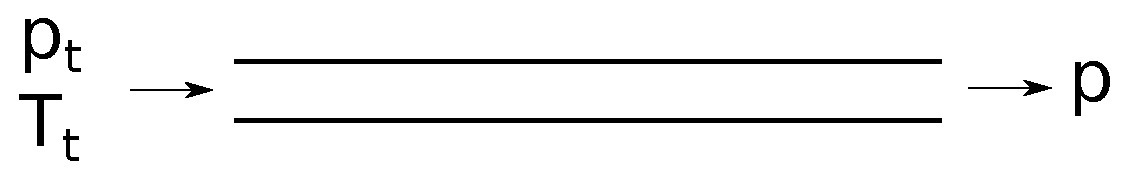
\includegraphics[width=0.9\hsize]{problem.eps}
\caption{Leitungssegment}
\label{fig:leitungssegment}
\end{figure}

\subsection{Randbedingungen}

Für Berechnungen über Rohrsegmente werden in der Strömungsmechanik übliche Grössen für die Randbedingungen verwendet:

Als Randbedingung am Austritt (in Abb.~\ref{fig:leitungssegment} rechts) wird der statische Druck $p$ verwendet, gelegentlich auch als Gegendruck bezeichnet, aber nicht zu verwechseln mit dem Staudruck.

Als Randbedingung am Eintritt (in Abb.~\ref{fig:leitungssegment} links) werden der Totaldruck $p_t$ und die Totaltemperatur $T_t$ verwendet, das entspricht den Zustandsgrössen des Mediums in Ruhe, bei Geschwindigkeit Null.

\subsection{Vernachlässigte Randbedingungen}

Es wird davon ausgegangen, dass die Temperatur von Medium und Umgebung ungefähr gleich ist und deshalb kein signifikanter Wärmeaustausch stattfindet.


\section{Grundgleichungen}

\begin{equation}
M = 1 + \frac{\gamma-1}{\gamma} \mathit{Ma}^2
\end{equation}

\end{document}
